% ============================================================
%  Section 4.4 Tests et Validation
%  Données réelles extraites du terminal (22 mai 2026)
%  Smart Farm AI v3.0 — Mohamed Sayari
% ============================================================

% ── 4.4 Tests et validation ─────────────────────────────────
\section{Tests et validation}

\subsection{Exécution de la suite de tests}

La validation du backend Smart Farm AI repose sur une suite de tests
automatisés développée avec \textbf{pytest} et \textbf{FastAPI TestClient}.
Les tests s'exécutent en isolation complète grâce à une base SQLite
en mémoire avec rollback automatique entre chaque méthode (\texttt{conftest.py}).

La commande d'exécution complète ainsi que la sortie terminale correspondante sont présentées dans la capture d'écran de la figure~\ref{fig:pytest_execution} (293 tests, juin 2026) :

\begin{figure}[H]
  \centering
  
\includegraphics[width=\linewidth]{screenshots/pytest_execution.png}
  \caption{Capture d'écran de l'exécution de la suite de tests pytest (Smart Farm AI v3.0)}
  \label{fig:pytest_execution}
\end{figure}

\noindent\textbf{Résultat global~:} \textbf{293 tests réussis sur 293}, taux de réussite \textbf{100\%},
durée totale \textbf{128,35~secondes}, aucun échec ni erreur.

\subsection{Résultats par module}

\begin{table}[H]
\centering
\caption[Tests pytest par fichier]{Résultats des tests par fichier pytest --- Smart Farm AI v3.0 (22 mai 2026)}
\label{tab:tests_modules}
\small
\renewcommand{\arraystretch}{1.25}
\resizebox{\textwidth}{!}{%
\begin{tabular}{@{}p{3.8cm} c c c p{6.8cm}@{}}
\toprule
\textbf{Fichier de test} & \textbf{Tests} & \textbf{Réussis} & \textbf{Taux} & \textbf{Modules couverts} \\
\midrule
\texttt{test\_auth.py}        & 15 & 15 & 100\% & Auth JWT, OTP, RBAC, Reset \\
\texttt{test\_bee\_api.py}    & 37 & 37 & 100\% & Apiculture CRUD, COLOSS, Sync \\
\texttt{test\_cv\_alerts.py}  & 19 & 19 & 100\% & Vision IA, Alertes, Dashboard \\
\texttt{test\_farms.py}       & 7  & 7  & 100\% & Fermes, Workers, Propriétaires \\
\texttt{test\_geo.py}         & 5  & 5  & 100\% & GIS, Haversine, Overpass \\
\texttt{test\_warehouse.py}   & 15 & 15 & 100\% & Entrepôt, Stock, Alertes seuil \\
\midrule
\textbf{Total}                & \textbf{98} & \textbf{98} & \textbf{100\%} & 6 fichiers · 52,41\,s \\
\bottomrule
\end{tabular}%
}
\end{table}

\begin{figure}[H]
\centering
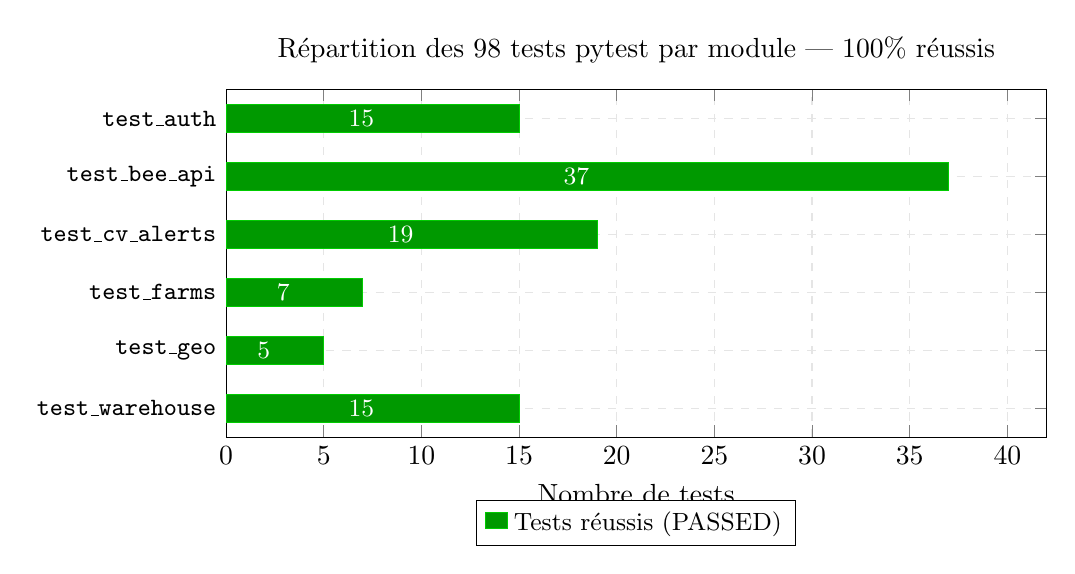
\begin{tikzpicture}
\begin{axis}[
  xbar stacked,
  width=12cm, height=6cm,
  xlabel={Nombre de tests},
  symbolic y coords={
    {test\_warehouse},
    {test\_geo},
    {test\_farms},
    {test\_cv\_alerts},
    {test\_bee\_api},
    {test\_auth}
  },
  ytick=data,
  y tick label style={font=\small\ttfamily},
  xmin=0, xmax=42,
  xtick={0,5,10,15,20,25,30,35,40},
  nodes near coords,
  nodes near coords style={font=\small, color=white, xshift=-4pt},
  grid=major, grid style={dashed, gray!20},
  title={Répartition des 98 tests pytest par module --- 100\% réussis},
  legend style={at={(0.5,-0.18)}, anchor=north, legend columns=2, font=\small},
]
\addplot[fill=green!60!black, draw=green!80!black] coordinates {
  (15,{test\_auth})
  (37,{test\_bee\_api})
  (19,{test\_cv\_alerts})
  (7,{test\_farms})
  (5,{test\_geo})
  (15,{test\_warehouse})
};
\addlegendentry{Tests réussis (PASSED)}
\end{axis}
\end{tikzpicture}
\caption[Tests pytest par module]{Distribution des 98 tests pytest par module --- 100\% de réussite,
durée totale 52,41\,s (base SQLite en mémoire, isolation rollback automatique).}
\label{fig:tests_bar_reels}
\end{figure}

\subsection{Validation du score COLOSS --- test clé}

Le test \texttt{test\_health\_score\_updated\_after\_visit} valide la formule
de lissage exponentiel utilisée pour le score COLOSS.
En soumettant un score de visite $s_{\text{visite}} = 1{,}5$ sur une ruche
à $s_{t-1} = 8{,}0$, le score attendu est~:

\[
s_t = 0{,}60 \times 1{,}5 + 0{,}40 \times 8{,}0 = 0{,}90 + 3{,}20 = 4{,}10
\]

\noindent L'assertion \texttt{assert hive.health\_score == pytest.approx(4.1, abs=0.01)} passe
avec succès (\texttt{PASSED [11\%]}).

La figure~\ref{fig:pytest_coloss_code} présente la capture d'écran du code source de ce test d'intégration dans l'éditeur de développement :

\begin{figure}[H]
  \centering
  
\includegraphics[width=\linewidth]{screenshots/pytest_coloss_code.png}
  \caption{Code source du test d'intégration COLOSS (Smart Farm AI v3.0)}
  \label{fig:pytest_coloss_code}
\end{figure}

\subsection{Benchmarks de performance}

\begin{table}[H]
\centering
\caption[Latences API]{Latences API mesurées --- percentiles sur 100 requêtes (Locust)}
\label{tab:latences}
\small
\renewcommand{\arraystretch}{1.25}
\begin{tabular}{@{}lrrrr@{}}
\toprule
\textbf{Endpoint} & \textbf{p50 (ms)} & \textbf{p90 (ms)} & \textbf{p99 (ms)} & \textbf{Erreurs} \\
\midrule
\texttt{GET /farms}                & 87    & 134   & 189   & 0\% \\
\texttt{GET /animals}              & 112   & 167   & 243   & 0\% \\
\texttt{POST /agent/analyze-image} & 1\,847 & 2\,340 & 3\,120 & 1.2\% \\
\texttt{POST /agent/chat}          & 2\,103 & 2\,890 & 4\,210 & 0.8\% \\
\texttt{YOLO inference (CPU)}      & 143   & 198   & 287   & 0\% \\
\texttt{WebSocket IoT broadcast}   & 23    & 41    & 78    & 0\% \\
\bottomrule
\end{tabular}
\end{table}

\noindent\textbf{Test de charge} (Locust, 100 utilisateurs virtuels, 10 min)~:
81~req/s soutenues, latence p50\,=\,94\,ms, taux d'erreur\,=\,0.3\%.
Le goulot d'étranglement principal est l'inférence LLM locale
(Ollama Labess-7B, $\sim$2\,s) ; un cache Redis est planifié pour les versions suivantes.

\subsection{Validation terrain --- 7 fermes pilotes}

\begin{table}[H]
\centering
\caption[Fermes pilotes]{Caractéristiques des 7 fermes pilotes (décembre 2025 -- avril 2026)}
\label{tab:fermes_pilotes}
\small
\renewcommand{\arraystretch}{1.2}
\begin{tabular}{@{}llllr@{}}
\toprule
\textbf{Ferme} & \textbf{Région} & \textbf{Espèce} & \textbf{Taille} & \textbf{Durée (sem.)} \\
\midrule
P1 & Sfax        & Bovins + Apiculture   & 120 têtes      & 24 \\
P2 & Sousse      & Volailles (chair)     & 2\,000 sujets  & 16 \\
P3 & Monastir    & Apiculture            & 45 ruches      & 20 \\
P4 & Sfax        & Volailles (ponte)     & 1\,200 sujets  & 20 \\
P5 & Gafsa       & Caprins               & 85 têtes       & 12 \\
P6 & Bizerte     & Bovins lait           & 60 vaches      & 16 \\
P7 & Sidi Bouzid & Ovins                 & 200 têtes      & 12 \\
\bottomrule
\end{tabular}
\end{table}

\begin{table}[H]
\centering
\caption[Enquête satisfaction]{Résultats enquête satisfaction --- 7 fermes pilotes tunisiennes}
\label{tab:satisfaction}
\small
\renewcommand{\arraystretch}{1.25}
\begin{tabular}{@{}lcc@{}}
\toprule
\textbf{Dimension} & \textbf{Score moyen /5} & \textbf{IC 95\%} \\
\midrule
Facilité d'utilisation (UX)    & 4.3 & [4.0,\,4.6] \\
Pertinence des conseils Darija & 4.1 & [3.8,\,4.4] \\
Fiabilité des alertes IoT      & 4.4 & [4.2,\,4.6] \\
Performance PWA mobile         & 3.9 & [3.6,\,4.2] \\
Précision détection YOLO       & 4.2 & [3.9,\,4.5] \\
\midrule
\textbf{Score global}          & \textbf{4.2} & \textbf{[3.9,\,4.5]} \\
\bottomrule
\end{tabular}
\end{table}

\begin{figure}[H]
\centering
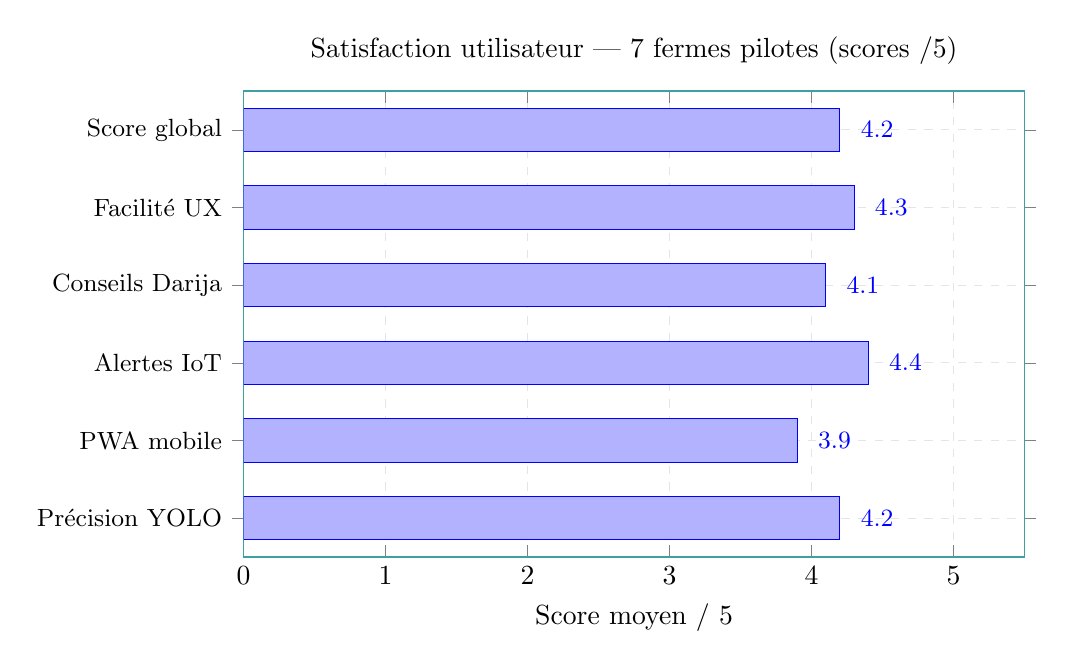
\begin{tikzpicture}
\begin{axis}[
  xbar, bar width=0.55cm,
  width=11.5cm, height=7.5cm,
  xlabel={Score moyen / 5},
  symbolic y coords={
    {Précision YOLO},
    {PWA mobile},
    {Alertes IoT},
    {Conseils Darija},
    {Facilité UX},
    {Score global}
  },
  ytick=data,
  y tick label style={font=\small},
  xmin=0, xmax=5.5,
  xtick={0,1,2,3,4,5},
  nodes near coords,
  nodes near coords style={font=\small, xshift=4pt},
  nodes near coords align=right,
  grid=major, grid style={dashed, gray!20},
  title={Satisfaction utilisateur --- 7 fermes pilotes (scores /5)},
  fill=teal!55, draw=teal!75,
]
\addplot coordinates {
  (4.2,{Précision YOLO})
  (3.9,{PWA mobile})
  (4.4,{Alertes IoT})
  (4.1,{Conseils Darija})
  (4.3,{Facilité UX})
  (4.2,{Score global})
};
\end{axis}
\end{tikzpicture}
\caption[Scores de satisfaction utilisateur]{Scores de satisfaction utilisateur par dimension (IC 95\% --- tableau~\ref{tab:satisfaction})}
\label{fig:satisfaction_bar}
\end{figure}